\chapter{Analisi dei requisiti}\label{chap:AnalisiRequisiti}
\section{Requisiti funzionali}
Questa sezione è dedicata alla suddivisione dei dati raccolti in requisiti funzionali.
La tabella seguente suddivide i requisiti per area del progetto.
Insieme al requisito e alla sua descrizione è presente anche l'elenco
dei ruoli a cui esso è rivolto.
\newpage
\begin{figure}[H]
    \centering
    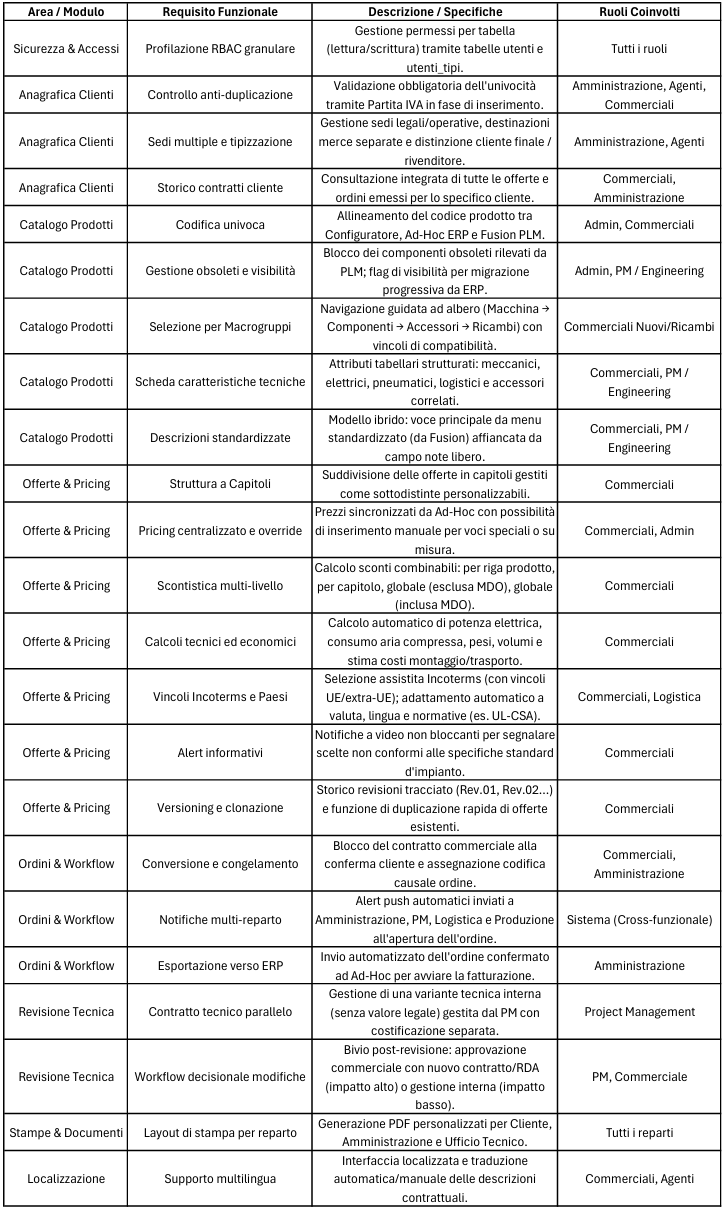
\includegraphics[width=0.8\linewidth]{Tabelle/RequisitiFunzionali.png}
    \caption{Requisiti funzionali raccolti.}\label{fig:Requisiti funzionali}
\end{figure}
\section{Requisiti non funzionali}
Questa sezione, a differenza della precedente raccoglie i requisiti non funzionali.
La tabella che seguirà, insieme al requisito stesso, raccoglie anche la sua categoria 
e la sua priorità all'interno dell'implementazione.
I requisiti sono ordinati per priorità.
\begin{figure}[h!]
    \centering
    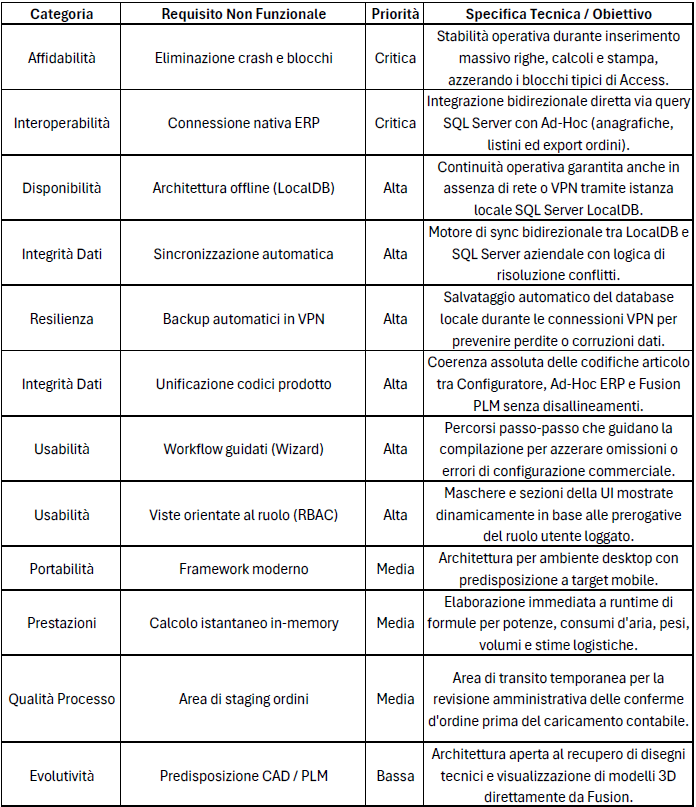
\includegraphics[width=0.9\linewidth]{Tabelle/RequisitiNonFunzionali.png}
    \caption{Requisiti non funzionali raccolti.}\label{fig:Requisiti non funzionali}
\end{figure}